\section{Manual}
\label{sec:manual}
\subsection{Dependencies \& Compilation}
Das Framework nutzt verschiedene Bibliotheken zum Testen, Generieren von Vektorbildern, Datenbankzugriff und das parsen von der Eingabe. Wir nutzen Maven um diese effizient und sauber zu implementieren und die Vorraussetzung ist Java 1.6.
\subsubsection{Dependancies}
\begin{itemize}
	\item junit\\
	Unit-Testing unter Java
	\item Batik SVG Toolkit\\
	Genutzt um SVG zu generieren, anzuzeigen und zu manipulieren
	\item SQLite4Java\\
	Um in die Datenbank zu schreiben
	\item Apache Commons CLI library\\
	Um die Konsoleneingabe standartisiert zu parsen und zu verarbeiten. Vereinfacht das schreiben von der Usage.
\end{itemize}

\subsection{Grafische Oberfläche}
Die Oberfläche ist dazu da Polygone zu generieren, den Shortest Path zu berechnen und diesen darzustellen.\\
\begin{center}
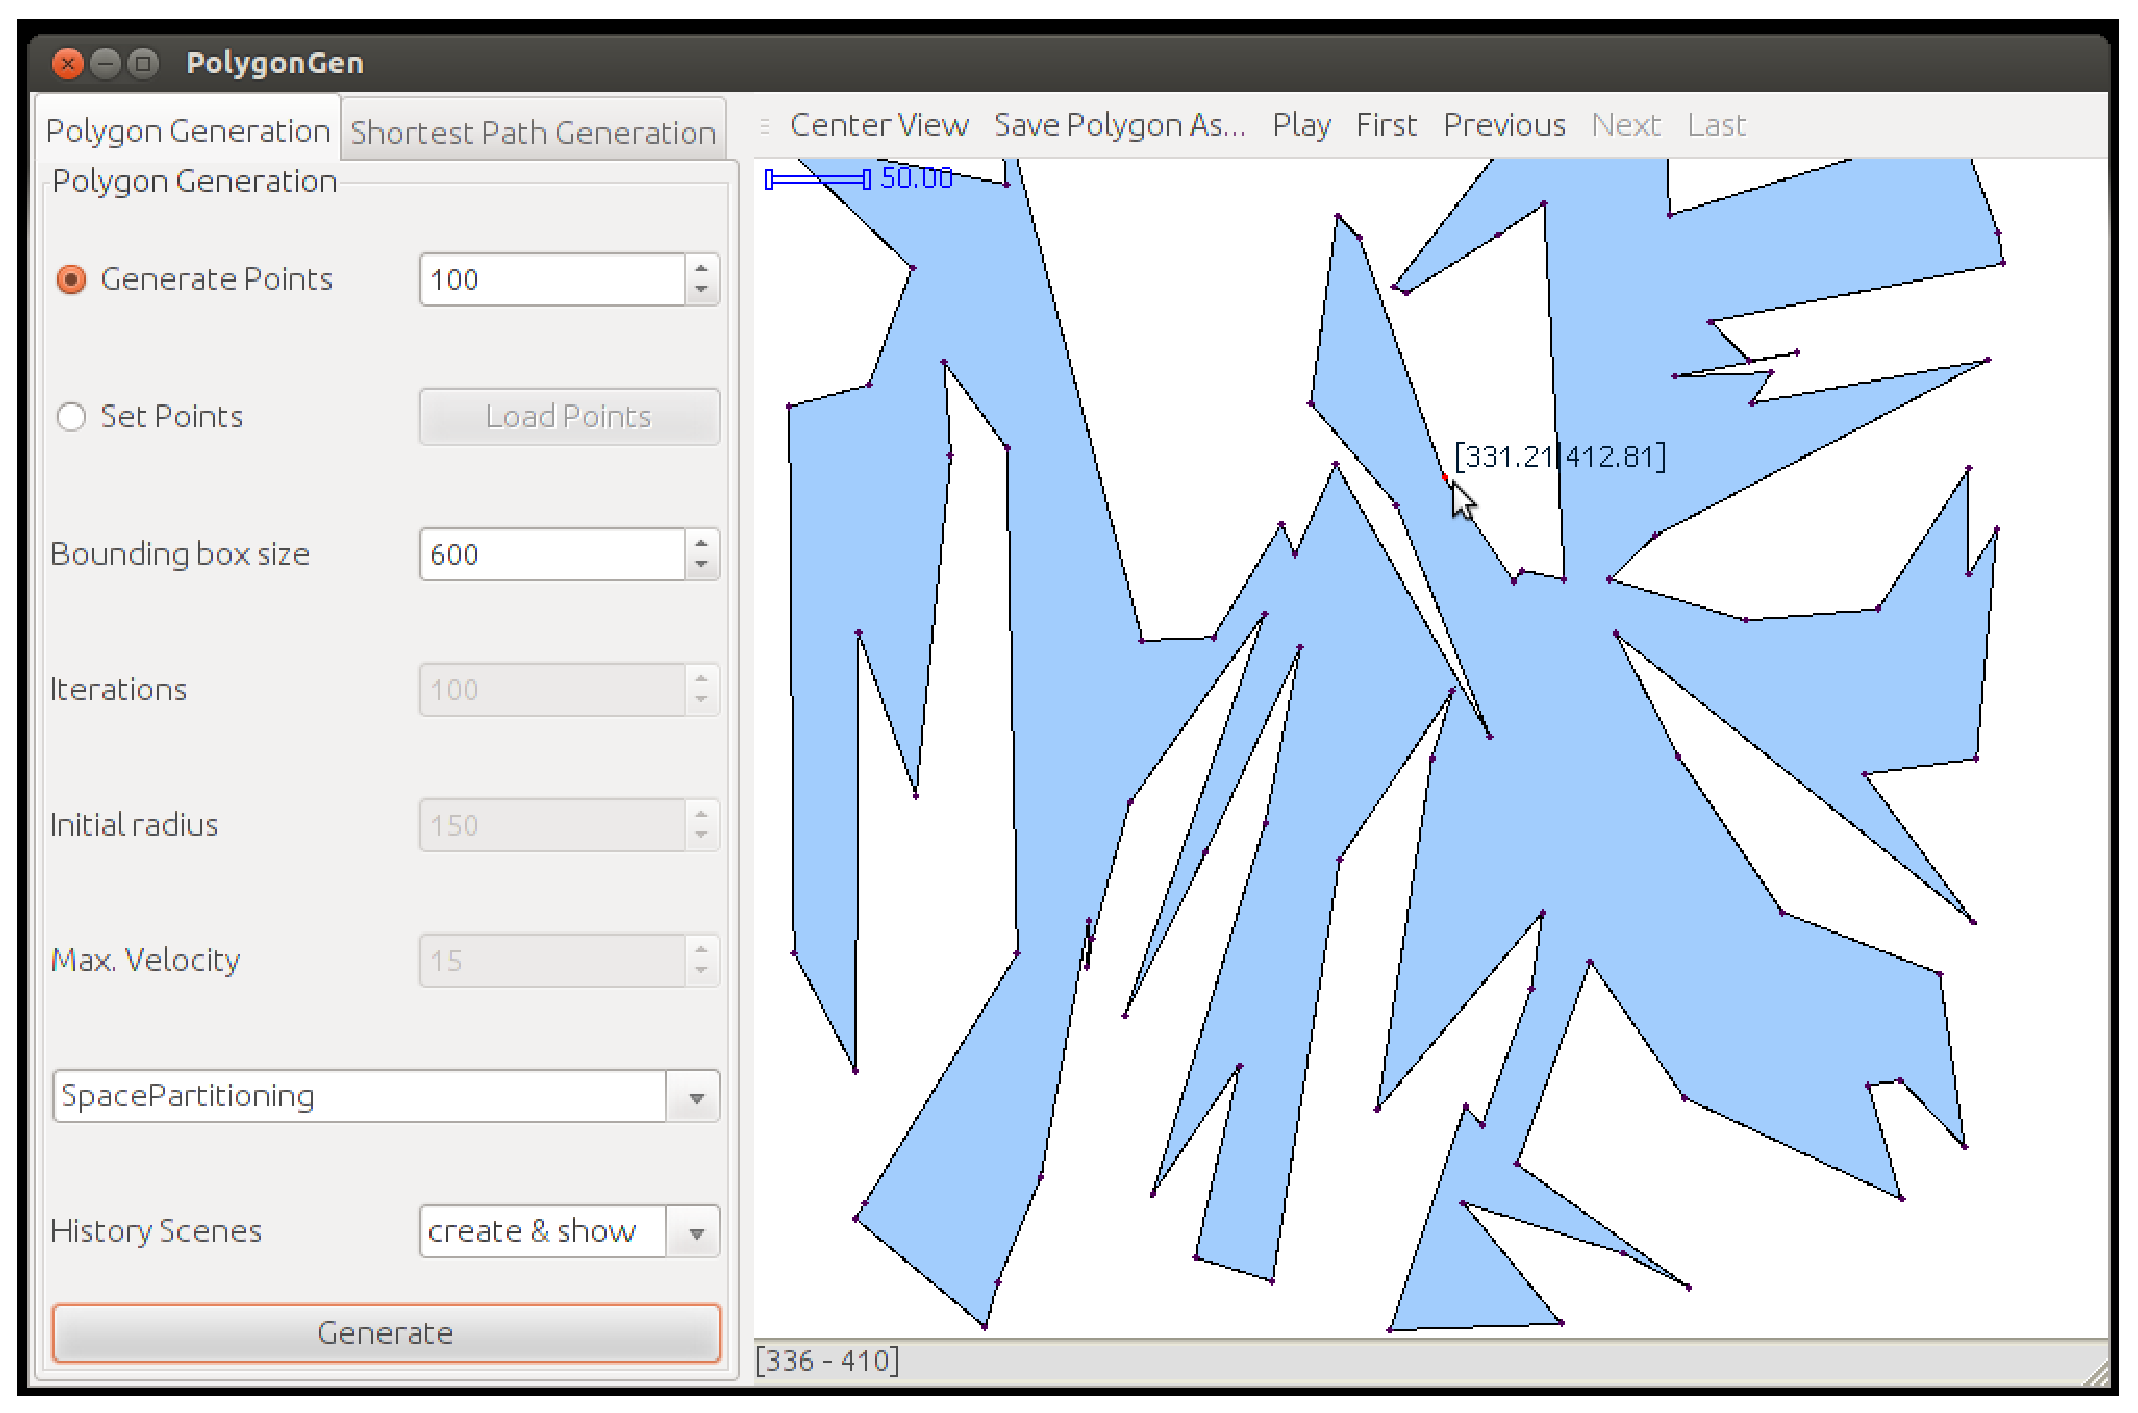
\includegraphics[width=0.7\textwidth]{img/GUI.eps}
\end{center}

\subsubsection{Funktionen}
\begin{itemize}
	\item Generierung von Polygonen
	\item Visualisierung der Polygone
	\item Manuelles setzen eines Polygons
	\item Schritt für Schritt-Visualisierung von der Erstellung des Polygons
	\item Zoomen und Bewegen in der Visualisierung des Polygons
	\item Anzeigen der Werte einzelner Polygone
	\item Berechnung des Shortest-Path
	\item Speichern des Polygons
\end{itemize}

\subsection{Kommandozeile}
Mit der Kommandozeile ist es möglich mehrere Polygone und deren Statistiken gleichzeitig zu erzeugen und diese in eine Ausgabedatei zu schreiben. Zusätzlich ist es möglich die Anzahl der Threads zu bestimmen für optimales paralleles Berechnen. Damit ist es möglich viele verschiedene Polygone mit den gleichen Parametern zu erzeugen. Die Parameter werden im \enquote{GNU-Stil} angegeben.\\
Um die Usage-Hilfe zu bekommen ruft man das Programm mit dem Parameter --help oder --usage auf. Folgender Block ist ein gekürzter Ausschnitt aus der Usage. Alle weiteren Parameter sind in der Usage näher erläutert.

\begin{code}
usage: run.sh [--algorithm <Algorithm>] [--boundingbox <boundingbox>]
       [--database <Database file>] [--help] [--number <Number of
       polygons>] [--output <Output path>] [--points <Number of points>]
       [--radius <circle radius>] [--runs <number of runs>] [--threads
       <Number of threads>] [--usage] [--velocity <velocity>]
-
Use with no arguments to show GUI, use --output and/or --database to start
batch-mode.
-
    --algorithm <Algorithm>         The algorithm to execute, specified by
                                    ID (Default: 0). Available algorithms:
                                    [0] SpacePartitioning
                                    [1] Permute & Reject
                                    [2] 2-Opt moves
                                    [3] RandomPolygonAlgorithm
                                    [4] Incremental Construction &
                                    Backtracking
                                    [5] ConvexHull
                                    [6] Velocity Virmani
                                    [7] SteadyGrowth
                                    [8] TwoPeasants

[...]
\end{code}

Die Nutzung ist einfach gestaltet und selbsterklärend. Bei der Generierung von 10 Polygonen mittels SpacePartitioning, 25 Punkten, 200 radius und der Ausgabe in den Ordner out, wäre der Aufruf: \enquote{run.sh --algorithm 0 --points 25 --radius 200 --output out}. Alle weiteren Aufrufe sind equivalent von der Syntax.